\documentclass[10.5pt,a4paper]{article}
\usepackage[margin=1.8cm]{geometry}
\usepackage{fontspec}
\setmainfont{DejaVu Sans}
\setmonofont{DejaVu Sans Mono}[Scale=0.9]
\usepackage{unicode-math}
\setmathfont{DejaVu Math TeX Gyre}
\usepackage{graphicx,enumitem,xcolor,booktabs}
\pagestyle{empty}
\setlength{\parindent}{0pt}
\setlist[enumerate]{label=\alph*),leftmargin=1.4em,itemsep=0pt}
\newcommand{\resp}[1]{\par\vspace{#1}}
\newcommand{\preg}[1]{\vspace{4pt}{\large\bfseries #1}\par\vspace{3pt}}
\begin{document}
{\Large\bfseries SI7011 · Evento evaluativo 3 · Parte A: leer la evidencia}\par\vspace{10pt}
\textbf{Nombre:} \rule{8cm}{0.4pt}\hfill\textbf{Documento:} \rule{4cm}{0.4pt}\par\vspace{8pt}
\textbf{Individual · sin computador ni apuntes · 45 minutos · 8 preguntas, 1 punto cada una.}
Respuestas cortas: una o dos frases por literal. Cuando la pregunta pide evidencia, cita un número leído de la figura o la tabla.
Todos los resultados son de corridas reales de los notebooks de las sesiones 05 y 06.
\vspace{6pt}\hrule\vspace{6pt}

\preg{1. Partir una serie de tiempo}
Jena Climate: ventanas de 120 horas, predecir la temperatura 24 horas después. La línea base dice «la temperatura en 24 h será la de ahora». El mismo MLP se entrena con dos particiones: \textbf{en el tiempo} (el primer 50\,\% entrena, el siguiente 25\,\% valida) o \textbf{barajada} (se barajan las ventanas del primer 75\,\% y se separan al azar). La prueba es siempre el último 25\,\% de la serie.\par\vspace{4pt}
\begin{center}
\begin{tabular}{lrr}
\toprule
MAE (°C) & validación & prueba \\
\midrule
línea base & 2.44 & 2.62 \\
MLP, partición en el tiempo & 2.50 & 2.67 \\
MLP, partición barajada & 2.30 & 2.57 \\
\bottomrule
\end{tabular}
\end{center}
\begin{enumerate}
\item Con la partición barajada, la validación promete que el MLP mejora a la línea base en 0.14 °C. ¿Cuánto la mejora en prueba? ¿Y con la partición en el tiempo, qué habría dicho la validación? Usa números de la tabla.\resp{2.0cm}
\item ¿Por qué barajar las ventanas antes de partir produce una fuga, si ninguna ventana aparece dos veces?\resp{1.6cm}
\item La temperatura media del bloque de entrenamiento es 8.82 °C y la de toda la serie 9.44 °C. ¿Con cuál se normaliza, y por qué?\resp{1.4cm}
\end{enumerate}

\newpage
\preg{2. El gradiente a lo largo de la ventana}
Tres modelos recurrentes entrenados en la misma tarea: una RNN simple, una LSTM y una GRU. La figura muestra cuánto cambia la pérdida con cada hora de la entrada.\par
\begin{center}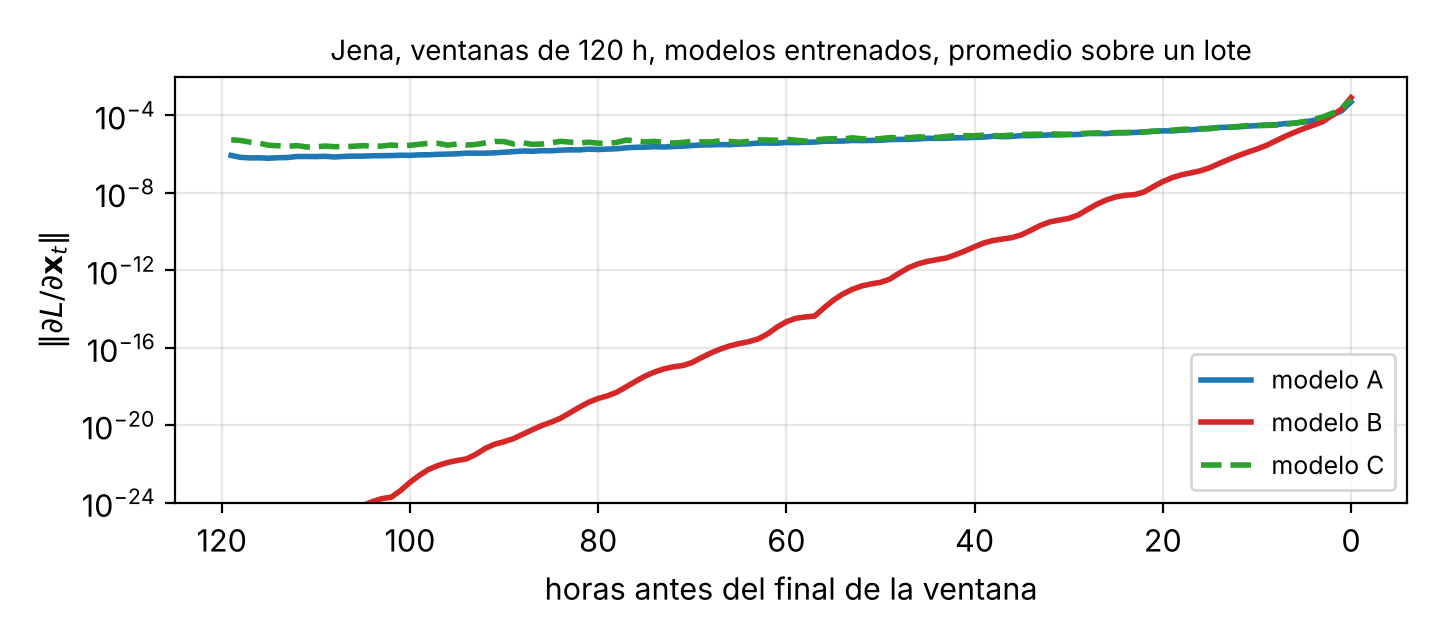
\includegraphics[width=0.74\linewidth]{fig1_gradiente.png}\end{center}
\begin{center}
\begin{tabular}{lrr}
\toprule
 & parámetros & MAE validación (°C) \\
\midrule
línea base & 0 & 2.44 \\
RNN, ventana de 120 h & 529 & 2.33 \\
RNN, ventana de 24 h & 529 & 2.33 \\
LSTM, ventana de 120 h & 2\,065 & 2.32 \\
GRU, ventana de 120 h & 1\,553 & 2.30 \\
\bottomrule
\end{tabular}
\end{center}
\begin{enumerate}
\item ¿Cuál curva es la RNN simple? Justifica con un valor leído de la figura y explica de dónde sale esa forma.\resp{2.2cm}
\item ¿Qué tiene la celda de la LSTM que evita esa forma?\resp{1.4cm}
\item La RNN da el mismo MAE con 120 h y con 24 h de ventana. ¿Qué dice eso, junto con la figura? Si la LSTM conserva el gradiente, ¿por qué casi no le gana a la RNN en esta tarea?\resp{2.4cm}
\end{enumerate}

\newpage
\preg{3. Barajar las palabras}
IMDB, 20\,000 reseñas de entrenamiento. Tres clasificadores: una \textbf{bolsa de embeddings} (promedio de los vectores de las palabras), una \textbf{CNN 1-D} y una \textbf{LSTM}. «Barajado» quiere decir que en el test se barajan las palabras de cada reseña, sin volver a entrenar.\par\vspace{4pt}
\begin{center}
\begin{tabular}{lrrr}
\toprule
 & parámetros & acc. test & acc. test barajado \\
\midrule
Modelo X & 1\,292\,545 & 0.841 & 0.796 \\
Modelo Y & 1\,280\,193 & 0.854 & 0.854 \\
Modelo Z & 1\,313\,473 & 0.826 & 0.807 \\
\bottomrule
\end{tabular}
\end{center}
\begin{enumerate}
\item ¿Cuál es la bolsa de embeddings? Justifica con la tabla y explica por qué ese resultado es exacto, no una casualidad.\resp{2.0cm}
\item ¿Qué dice este experimento sobre si clasificar el sentimiento de una reseña necesita un modelo que tenga en cuenta el orden?\resp{2.0cm}
\item Con embeddings GloVe preentrenados \textbf{congelados}, la bolsa da 0.753; con GloVe \textbf{ajustados} a IMDB, 0.859. ¿Por qué la diferencia, si los dos parten de los mismos vectores?\resp{2.0cm}
\end{enumerate}

\preg{4. El cuello de botella del seq2seq}
Fechas en palabras a formato ISO: «el primero de mayo de 2 0 2 6» → \texttt{2026-05-01}. El encoder y el decoder son GRU de tamaño $d$. Exactitud por posición de la salida:\par\vspace{4pt}
\begin{center}\small\setlength{\tabcolsep}{4pt}
\begin{tabular}{lrrcccccccccc}
\toprule
 & parám. & exacta & \multicolumn{4}{c}{año} & \texttt{-} & \multicolumn{2}{c}{mes} & \texttt{-} & \multicolumn{2}{c}{día} \\
\midrule
sin atención, $d=24$ & 14\,204 & 0.004 & 1.00 & 1.00 & 0.98 & 0.95 & 1.00 & 0.76 & \textbf{0.15} & 1.00 & \textbf{0.32} & \textbf{0.09} \\
sin atención, $d=96$ & 99\,020 & 1.000 & 1.00 & 1.00 & 1.00 & 1.00 & 1.00 & 1.00 & 1.00 & 1.00 & 1.00 & 1.00 \\
con atención, $d=24$ & 16\,220 & 1.000 & 1.00 & 1.00 & 1.00 & 1.00 & 1.00 & 1.00 & 1.00 & 1.00 & 1.00 & 1.00 \\
\bottomrule
\end{tabular}
\end{center}
\begin{enumerate}
\item Sin atención, ¿qué recibe el decoder del encoder? Con eso, explica por qué $d=24$ falla y $d=96$ no.\resp{2.0cm}
\item Los errores se concentran en el día y el mes. Mira el orden de la frase de entrada: ¿por qué esos y no el año?\resp{1.8cm}
\item La atención agrega menos de 2\,100 parámetros y resuelve la tarea con $d=24$. ¿Qué cambia en lo que el decoder puede leer?\resp{1.6cm}
\end{enumerate}

\newpage
\preg{5. Máscaras y posiciones}
La misma capa de autoatención sobre «me senté en el banco», rellenada con dos \texttt{[PAD]} para formar un lote. Cada mapa muestra los pesos de atención $\alpha_{ij}$ con una máscara distinta: ninguna, de relleno, o causal más relleno.\par
\begin{center}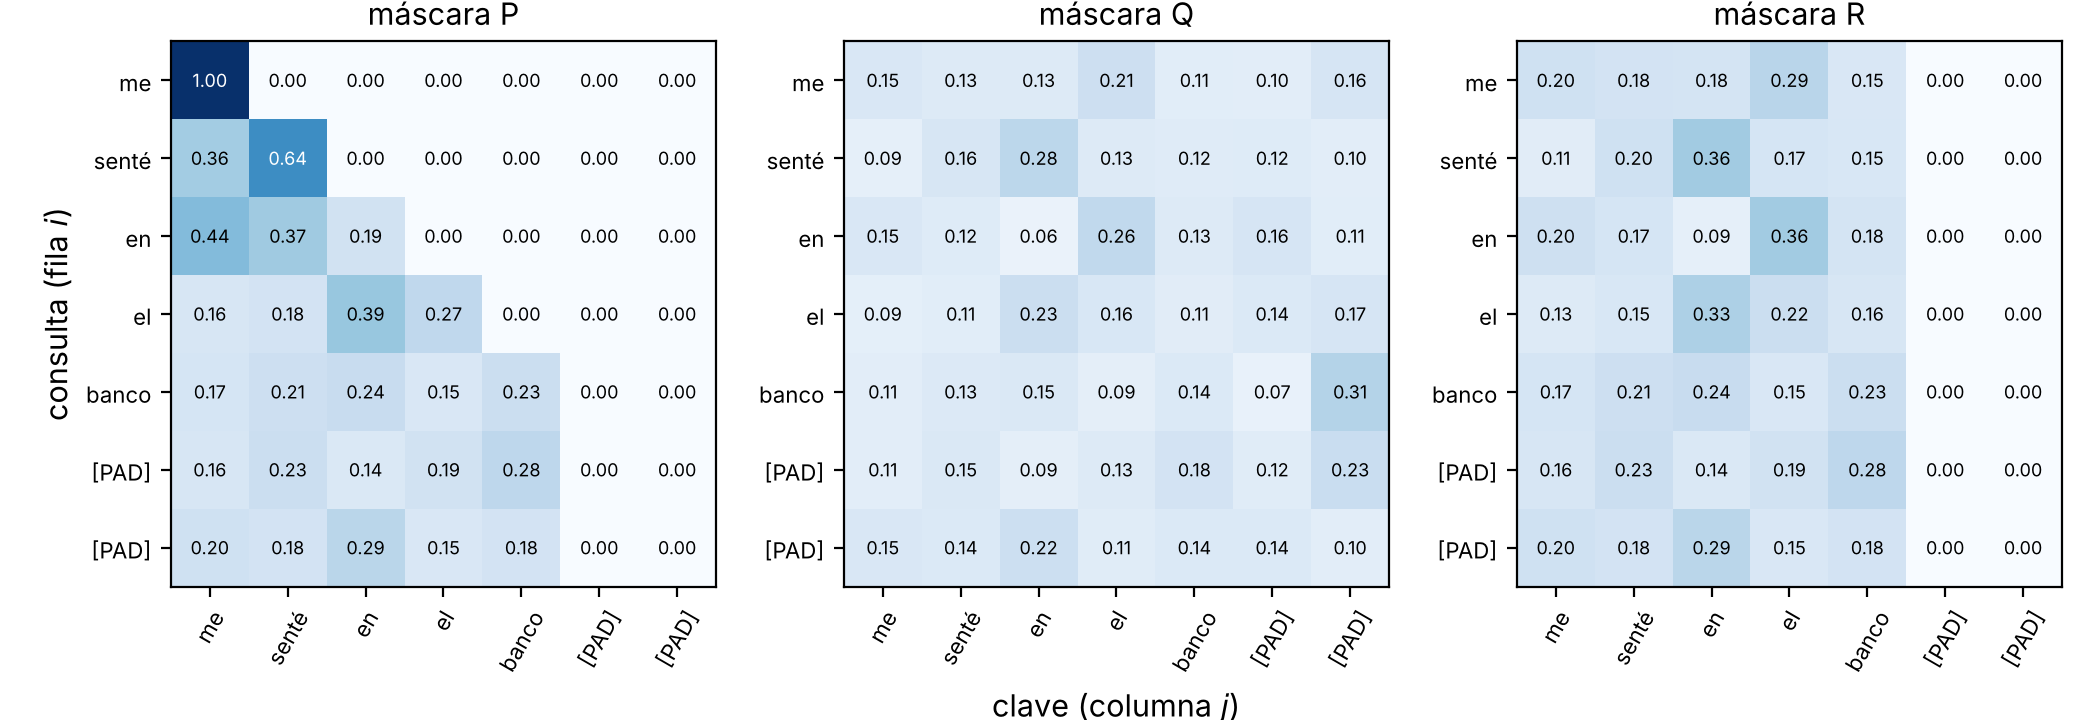
\includegraphics[width=\linewidth]{fig2_mascaras.png}\end{center}
\begin{enumerate}
\item Asigna P, Q y R. Justifica cada una con lo que ves en el mapa.\resp{2.2cm}
\item ¿Qué problema produce Q en un lote con frases de distinto largo?\resp{1.4cm}
\item Sin embeddings de posición, se reordenan las cinco palabras y se pasan por la misma capa: las salidas son las mismas, en el nuevo orden (diferencia máxima $9\cdot10^{-8}$). Con posiciones, la diferencia es 0.23. ¿Por qué? ¿Qué consecuencia tiene para «el perro mordió al hombre» y «el hombre mordió al perro»?\resp{2.4cm}
\end{enumerate}

\newpage
\preg{6. El Transformer de las fechas y su costo}
La misma tarea de la pregunta 4 con un Transformer encoder-decoder, $d = 64$, 245\,964 parámetros.\par\vspace{4pt}
\begin{center}\small
\begin{tabular}{lrcccccccccc}
\toprule
 & exacta & \multicolumn{4}{c}{año} & \texttt{-} & \multicolumn{2}{c}{mes} & \texttt{-} & \multicolumn{2}{c}{día} \\
\midrule
con posición & 0.999 & 1.00 & 1.00 & 1.00 & 1.00 & 1.00 & 1.00 & 1.00 & 1.00 & 1.00 & 1.00 \\
sin posición & 0.660 & 0.99 & 0.99 & \textbf{0.72} & \textbf{0.67} & 1.00 & 1.00 & 1.00 & 1.00 & 0.95 & 0.90 \\
\bottomrule
\end{tabular}
\par\vspace{6pt}
\begin{tabular}{lrrrrr}
\toprule
longitud $T$ & 128 & 256 & 512 & 1\,024 & 2\,048 \\
\midrule
memoria de la matriz de atención (MB) & 0.25 & 1 & 4 & 16 & 64 \\
\bottomrule
\end{tabular}
\end{center}
\begin{enumerate}
\item Sin posición, el modelo falla sobre todo en las dos últimas cifras del año, que en la entrada vienen como dígitos sueltos («2 0 2 6»), y nunca en el mes, que viene como palabra («mayo»). Explica por qué.\resp{2.2cm}
\item ¿Por qué factor crece la memoria de la atención cuando $T$ se duplica? ¿Cuánta ocuparía con $T = 4\,096$?\resp{1.4cm}
\item ¿Cuántos parámetros tienen $W_Q$, $W_K$, $W_V$ y $W_O$ (con sesgo) de una capa de atención con $d = 64$? ¿Cambia ese número con $T$?\resp{1.4cm}
\end{enumerate}

\newpage
\preg{7. La pérdida del ajuste supervisado}
Un par pregunta–respuesta de Dolly en la plantilla de chat. Cada barra es la pérdida de predecir ese token con el modelo base, antes de ajustarlo.\par
\begin{center}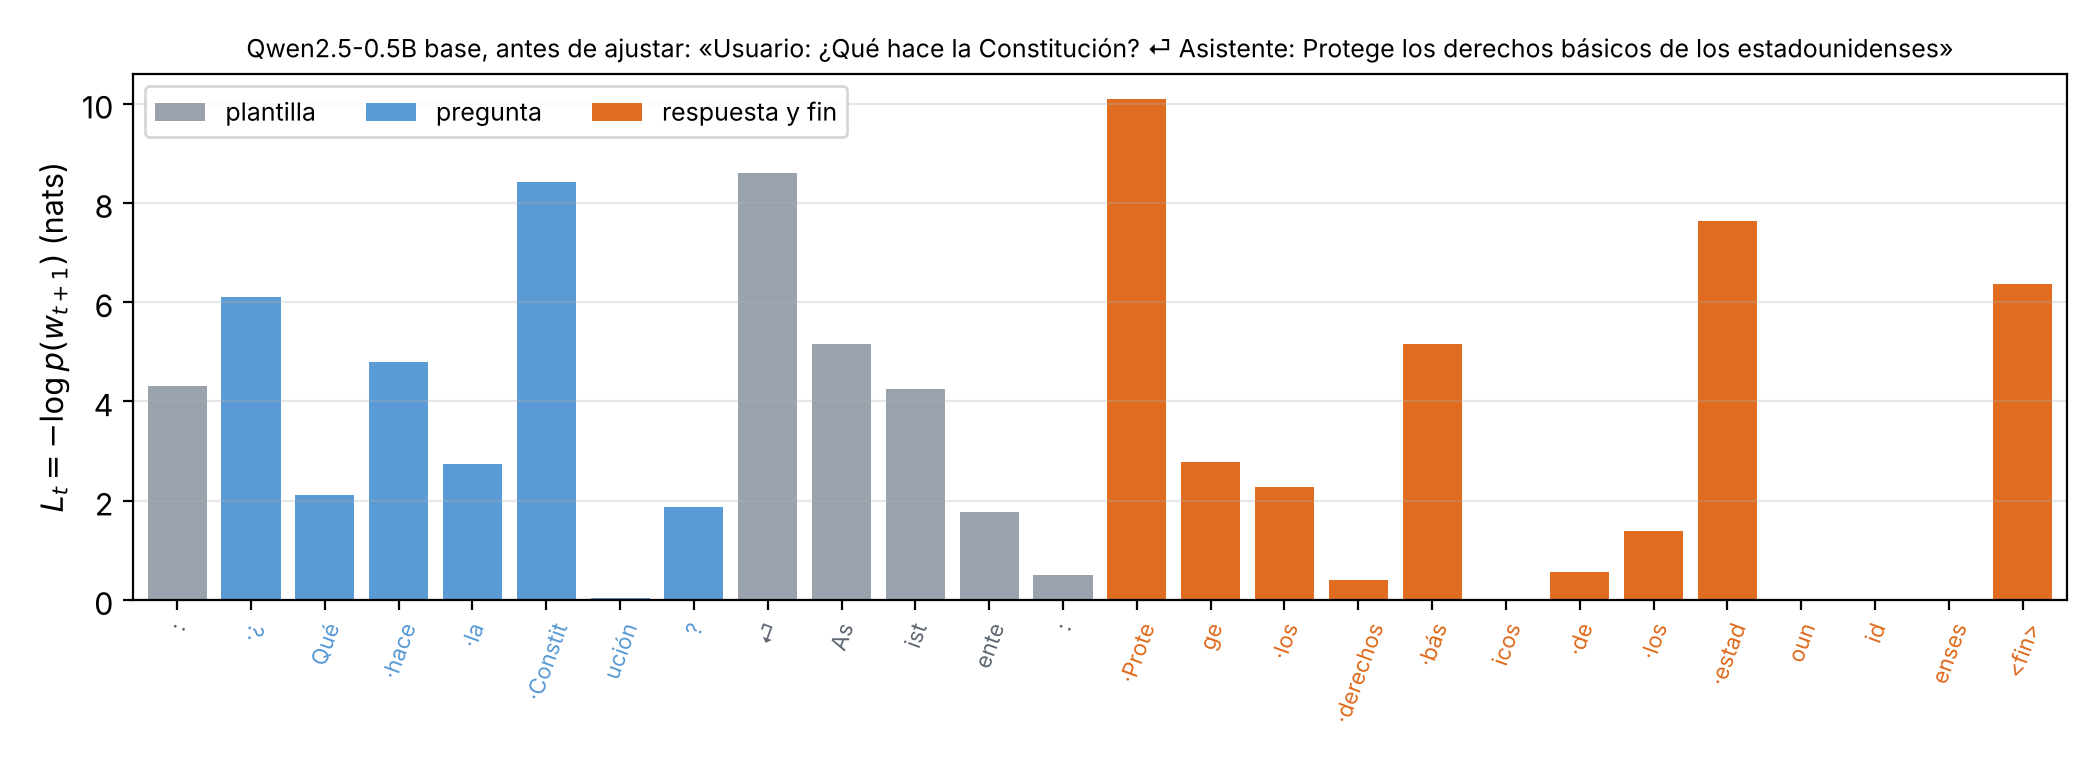
\includegraphics[width=\linewidth]{fig3_perdida.png}\end{center}
\begin{enumerate}
\item En el ajuste supervisado (SFT), ¿qué barras entran en la pérdida $J$ y por qué las otras no? El promedio de las 26 barras es 3.36; el de las que cuentan, 2.82. ¿Cuál de los dos números optimiza el SFT?\resp{2.2cm}
\item Después de 250 pasos de LoRA, la $J$ de validación pasa de 2.060 a 1.903 nats por token. Traduce los dos valores a perplejidad ($e^{2.06}\approx7.8$, $e^{1.90}\approx6.7$) y explica qué significa ese número.\resp{1.8cm}
\item De 12 preguntas, el modelo base se detiene solo en 2; después del ajuste, en 9. Pero ahora responde «Ballena: aves». ¿Qué aprendió el modelo en 250 pasos, y qué no?\resp{1.8cm}
\item ¿Se puede comparar esta $J$ con la de otro modelo que usa otro tokenizador? ¿Por qué?\resp{1.4cm}
\end{enumerate}

\newpage
\preg{8. Elegir cómo usar un modelo preentrenado}
IMDB con solo \textbf{2\,000} reseñas de entrenamiento, 2\,000 de test, GPU T4.\par\vspace{4pt}
\begin{center}
\setlength{\tabcolsep}{4pt}\begin{tabular}{lrrrr}
\toprule
 & acc. test & entrenables & tiempo & memoria \\
\midrule
LSTM desde cero & 0.778 & 4.2 M & 15 s & 0.7 GB \\
DistilBERT congelado + sonda logística sobre \texttt{[CLS]} & 0.801 & 769 & 13 s & 1.0 GB \\
DistilBERT ajustado completo & 0.886 & 67 M & 40 s & 2.2 GB \\
DistilBERT + LoRA ($r=8$, $W_Q$ y $W_V$) + cabeza & 0.891 & 740 k & 34 s & 1.5 GB \\
\bottomrule
\end{tabular}
\end{center}
\begin{enumerate}
\item La LSTM entrena más parámetros que LoRA y queda 11 puntos por debajo. ¿Qué es lo que compra la exactitud, si no son los parámetros entrenables?\resp{1.8cm}
\item ¿Por qué el modelo congelado con sonda queda tan por debajo de los ajustados, si usa el mismo DistilBERT?\resp{1.8cm}
\item Una clínica tiene 800 notas clínicas en español etiquetadas para \textbf{tres} tareas distintas y una GPU de 16 GB. ¿Qué estrategia eliges y qué cambiarías del experimento de arriba? Nombra la línea base contra la que la compararías.\resp{3.0cm}
\end{enumerate}

\end{document}
